\chapter{Der kleine Kapiteltest}
	\blindtext

\section{Unterkapitel mit Blindtext und Bild}
	\blindtext
	
	
	\begin{figure}
		\centering
		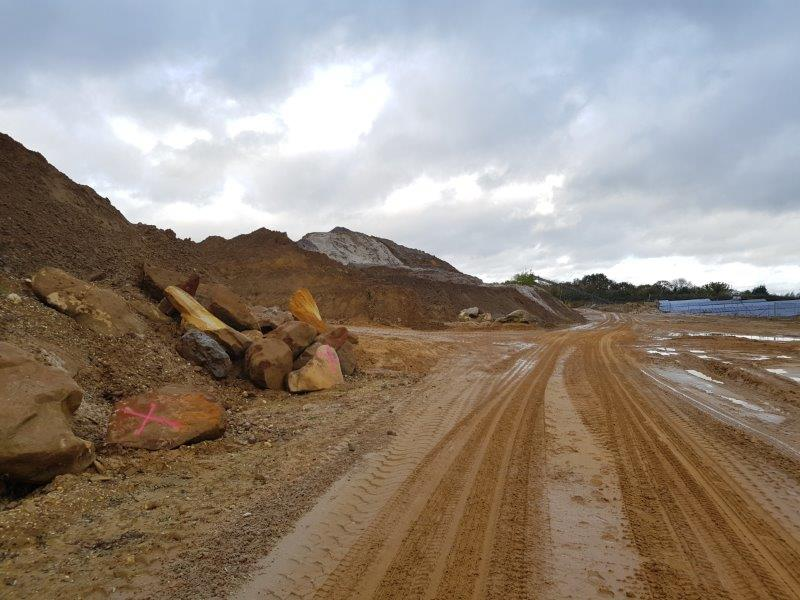
\includegraphics[width=0.7\linewidth]{20191112_111105.jpg}  % picked from the defined standard folder 'figures/'
		\caption{Nievelsteiner Steinbruch}
		\label{fig:20191112111105}
	\end{figure}


\section{Unterkapitel mit Beispielen}
	Griechische Buchstaben können direkt eingetippt werden. So kann α anstatt \$\textbackslash alpha\$ (o.~ä.) im Fließtext verwendet werden.
	
	Es folgt ein Beispiel für die Verwendung von Abkürzungen:
	\begin{itemize}
		\item erstes auftreten der Abkürzung: \ac{ufo}
		\item zweites auftreten der Abkürzung: \ac{ufo}
		\item volle Ausgabe der Abkürzung: \acf{ufo}
		\item Langfassung der Abkürzung: \acl{ufo}
		\item kurzfassung der Abkürzung: \acs{ufo}
	\end{itemize}
	
	Noch ein weiteres Beispiel für die Verwendung von Abkürzungen:
	\begin{itemize}
		\item erstes auftreten der Abkürzung: \ac{3ax}
		\item zweites auftreten der Abkürzung: \ac{3ax}
	\end{itemize}
	
	Im folgenden wird gezeigt, dass die deutsche Notation für die Darstellung von Zahlen verwendet wird. Dabei ist das ``,'' das Dezimaltrennzeichen und ein ``.'' ein Tausendertrennzeichen, wobei der Punkt durch ein halbes Leerzeichen ersetzt wird.\\
	\begin{math}
		1 + 2,3\cdot 4.500 - 8.000,500654 = 54,3 \alpha
	\end{math}
	
	Hier wird die Nummerierung von Formeln gezeigt:
	\begin{equation}
		a=b
	\end{equation}
	
	\begin{table}
		\caption{Einkommen abhängig vom Studium}
		\label{tbl:testtest}
		\centering
		\begin{tabular}{lrr} 
			\toprule
			Fach & Dauer & Einkommen (€)\\ 
			\midrule 
			Bauing & 10 & $45.000$ \\
			WirtIng & 6 & $65.000$ \\
			AngewGeoW & 8 & $35.000$\\ 
			\bottomrule
		\end{tabular}
	\end{table}


\subsection{Unterunterkapitel 1}
	Hier werden nun ein paar Zitationen vorgestellt. Es gibt solche im Text von \textcite{alam_effects_2014} und jene die am Ende eines Abschnitts stehen. \parencites{bailey_technology_2018}{alam_effects_2014}{dassault_systemes_abaqus_2017}{dassault_systemes_abaqus_2019}
	
	\blindtext \parencite{alireza_hassanzadegan_thermomechanical_2012}